\documentclass[11pt]{article}

% Layout & header
\usepackage[margin=1in,headheight=16pt]{geometry}
\usepackage{fancyhdr}
\usepackage{parskip}
\usepackage{tcolorbox}

% Math, figures, lists
\usepackage{amsmath,amssymb,mathtools}
\usepackage{graphicx}
\usepackage{float}
\usepackage{enumitem}
\usepackage{booktabs}

% Code (Python default; switch to Matlab in listings where needed)
\usepackage[dvipsnames]{xcolor}
\usepackage{listings}

% --- Fix indentation and alignment for listings inside environments ---
\makeatletter
\lst@AddToHook{EveryDisplay}{\parindent=0pt}
\makeatother

\lstdefinestyle{python}{
	language=Python,
	basicstyle=\ttfamily\small,
	keywordstyle=\color{NavyBlue}\bfseries,
	commentstyle=\color{ForestGreen}\itshape,
	stringstyle=\color{BrickRed},
	numbers=left,
	numberstyle=\tiny,
	numbersep=8pt,
	frame=single,
	breaklines=true,
	columns=fullflexible,
	showstringspaces=false,
	xleftmargin=0pt,
	framexleftmargin=0pt,
	aboveskip=0.8em,
	belowskip=0.8em
}
\lstset{style=python}

% Hyperlinks (load last)
\usepackage{hyperref}

% Header content
\pagestyle{fancy}
\fancyhf{}
\fancyhead[L]{October 8th 2025}
\fancyhead[C]{ECE 506: Homework \#3}
\fancyhead[R]{Scott Nguyen}
\renewcommand{\headrulewidth}{0.4pt}

\begin{document}
	
	\textbf{ECE 506: Homework \#3: Fundamentals of 1D Unconstrained Optimization Methods}
	
	\vspace{1em}
	To get help with the homework, please join the Saturday morning discussion sessions starting at 9am at:
	\url{https://unm.zoom.us/j/99977790315}.
	
	\noindent\textbf{Reference:} \\
	\emph{Numerical Methods for Unconstrained Optimization and Nonlinear Equations} by J.E. Dennis, Jr. and R.B. Schnabel, \\
	Classics in Applied Mathematics, SIAM 1996.
	
	\noindent\textbf{Matlab code:} \\
	Download the code from:\\ \url{https://github.com/pattichis/opt/blob/main/Code-for-Hwk-from-2012-Opt-1D.zip}.
	
	\noindent\textbf{Coding examples:} \\
	For all of your homework solutions, you must provide:
	\begin{enumerate}
		\item Documented source code,
		\item Plots, and
		\item Discussion.
	\end{enumerate}
	In the discussion, examples are sketched. For your solutions, you must provide working coding examples unless the problem specifically asks for a sketch.\\
	\textit{All code listings that previously appeared inline have been moved to Appendix~A at the end of this document.}
	
	\newpage
	% =================================================================
	\section*{Problem \#1. Bisection}
	
	\noindent\textbf{Helper Function (shown once):} We use \texttt{run\_case} to call \texttt{bisection} and plot/save via \texttt{visualize\_bisection\_results}.\\
	\emph{(Code moved to Appendix~A.)}
	
	\begin{enumerate}[label=1(\alph*)]
		
		\item \textbf{Root finding for linear functions.}
		\begin{enumerate}[label=\roman*)]
			
			\item Provide a coding example that demonstrates everything working correctly.\\
			\textbf{Solution.}\\
			\textit{MATLAB call:} \emph{(See Appendix~A.)}
			
			\begin{figure}[H]\centering
				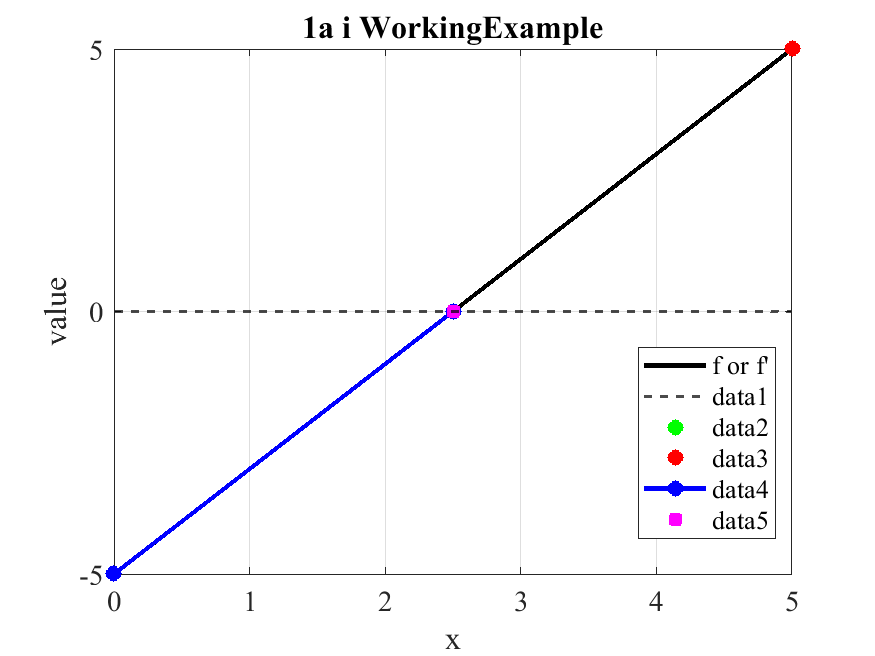
\includegraphics[width=0.78\linewidth]{plots/1a_i_WorkingExample.png}
				\caption{Linear, bracketed root (\(f(x)=2x-5\)) with labeled \(y=0\) reference.}
			\end{figure}
			
			\item Provide a coding example that demonstrates failure if possible. If not possible, discuss why failure is not possible.\\
			\textbf{Solution.}\\
			\textit{MATLAB call:} \emph{(See Appendix~A.)}
			
			\begin{figure}[H]\centering
				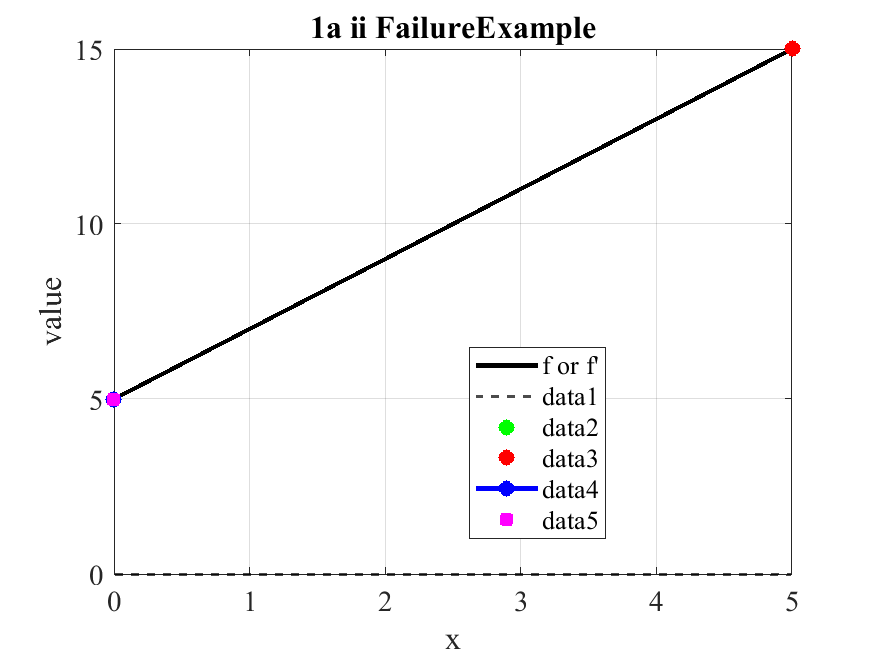
\includegraphics[width=0.78\linewidth]{plots/1a_ii_FailureExample.png}
				\caption{No sign change on \([0,5]\) for \(f(x)=2x+5\) \(\Rightarrow\) bisection cannot start.}
			\end{figure}
			
		\end{enumerate}
		
		\item \textbf{Root finding for quadratics.}
		\begin{enumerate}[label=\roman*)]
			
			\item Provide a coding example that demonstrates everything working correctly.\\
			\textbf{Solution.}\\
			\textit{MATLAB call:} \emph{(See Appendix~A.)}
			
			\begin{figure}[H]\centering
				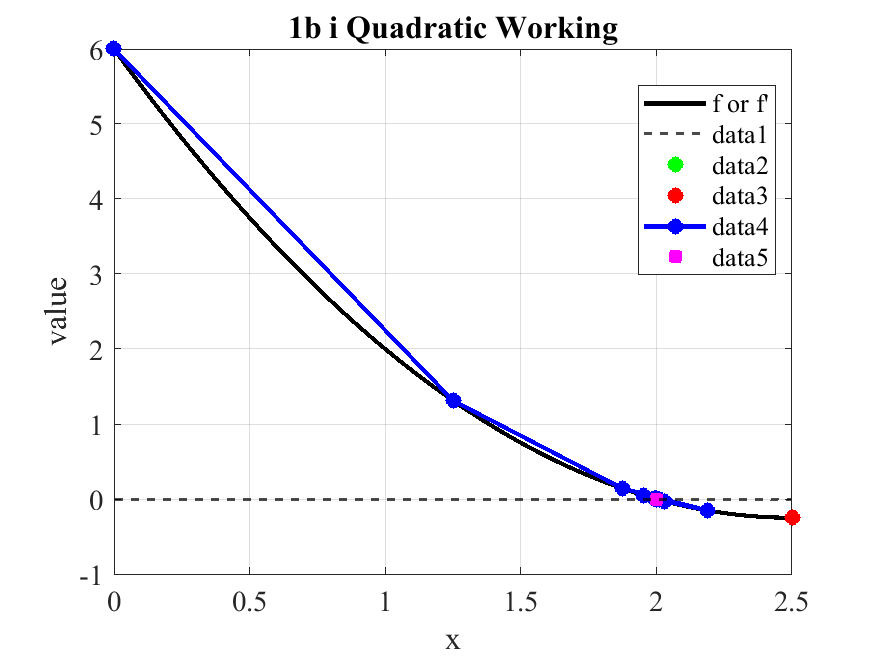
\includegraphics[width=0.78\linewidth]{plots/1b_i_Quadratic_Working.png}
				\caption{Quadratic with roots at \(x=2,3\); interval \([0,2.5]\) brackets \(x=2\).}
			\end{figure}
			
			\item Provide a coding example that demonstrates failure if possible. If not possible, discuss why failure is not possible.\\
			\textbf{Solution.}\\
			\textit{MATLAB call:} \emph{(See Appendix~A.)}
			
			\begin{figure}[H]\centering
				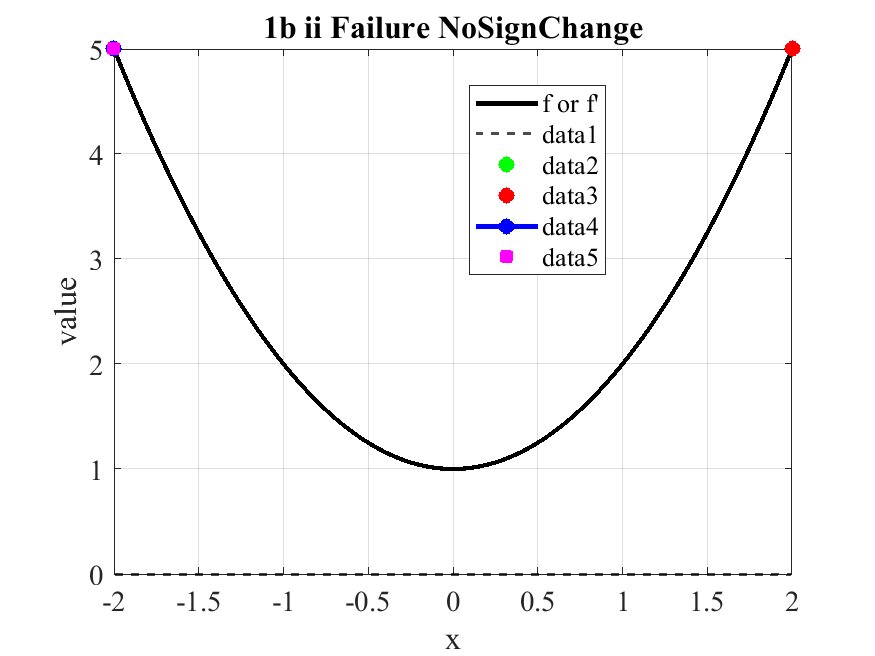
\includegraphics[width=0.78\linewidth]{plots/1b_ii_Failure_NoSignChange.png}
				\caption{\(x^2+1>0\) on \([-2,2]\): no sign change, bisection cannot start.}
			\end{figure}
			\begin{figure}[H]\centering
				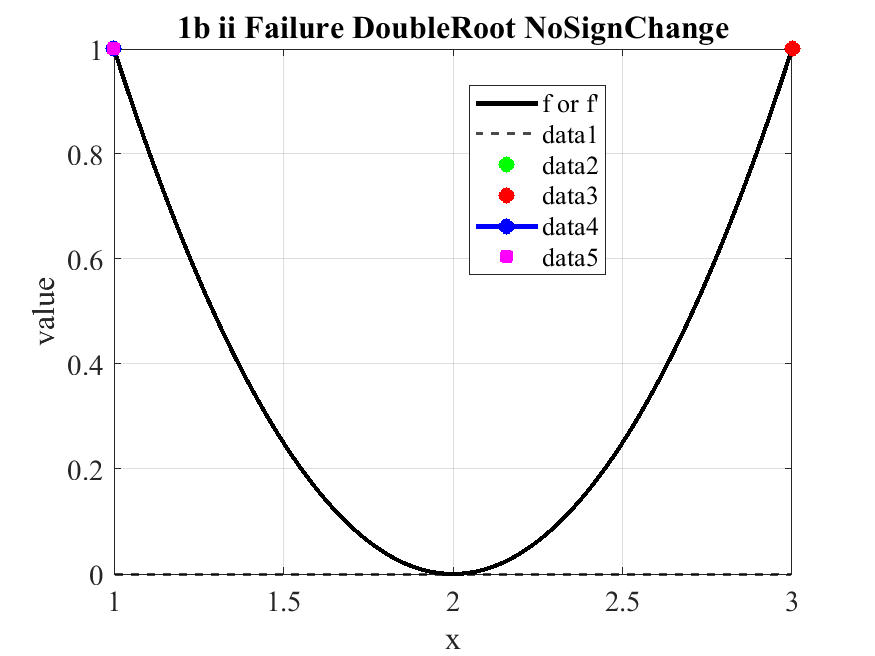
\includegraphics[width=0.78\linewidth]{plots/1b_ii_Failure_DoubleRoot_NoSignChange.png}
				\caption{Double root at \(x=2\): \(f(a),f(b)>0\) so standard bisection won’t detect it.}
			\end{figure}
			
		\end{enumerate}
		
		\item \textbf{Root finding for continuous functions.}
		\begin{enumerate}[label=\roman*)]
			
			\item What are the minimum requirements for bisection to work?\\
			\textbf{Solution.}\\
			\(1)\) \(f\) continuous on \([a,b]\);\quad \(2)\) \(f(a)\cdot f(b) < 0\) (opposite signs), which guarantees a root in \((a,b)\) by the Intermediate Value Theorem.
			
			\item Sketch an example.\\
			\textbf{Solution.}\\
			\textit{MATLAB call:} \emph{(See Appendix~A.)}
			
			\begin{figure}[H]\centering
				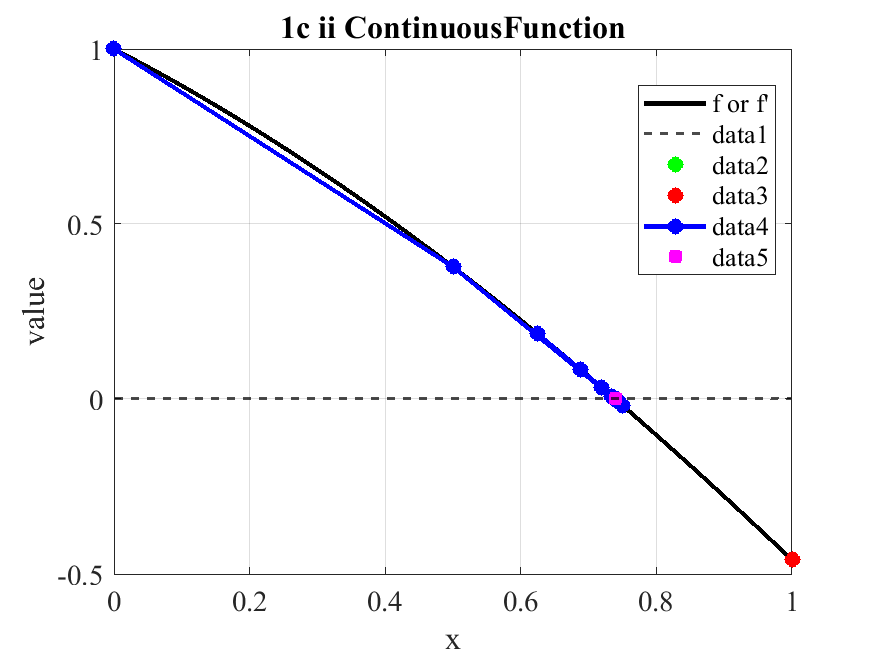
\includegraphics[width=0.78\linewidth]{plots/1c_ii_ContinuousFunction.png}
				\caption{\(f(x)=\cos x - x\) on \([0,1]\): continuous with a sign change; bisection converges.}
			\end{figure}
			
		\end{enumerate}
		
		\item \textbf{Convergence property for root finding.}\\
		Assume that all conditions are satisfied. Derive an expression for the root interval after $n$ steps of the algorithm.
		
		\textbf{Solution.}
		After $n$ steps, the bracket length is \(|I_n|=(b-a)/2^n\). If $x_n$ is the midpoint, then \(|x_n-x^\star|\le (b-a)/2^{n+1}\). Hence it suffices that
		\(n \ge \lceil \log_2\!\frac{b-a}{\varepsilon}\rceil - 1\) to ensure \(|x_n-x^\star|\le\varepsilon\).
		
	\end{enumerate}
	
	% =================================================================
	\newpage
	\section*{Problem \#2. Bisection applied to $f'(x)=0$}
	
	\noindent Repeat Problem \#1 for solving $f'(x)=0$. For this problem, success or failure refers to minimizing $f(x)$.\\
	\emph{(All code moved to Appendix~A.)}
	
	\begin{enumerate}[label=\textbf{\arabic*)}, leftmargin=2.2em]
		
		\item \textbf{Root finding for linear functions (on $f'(x)$).}
		\begin{enumerate}[label=\roman*)]
			
			\item Provide a coding example that demonstrates everything working correctly.\\
			\textbf{Solution.}\\
			\textit{MATLAB call:} \emph{(See Appendix~A.)}
			
			\begin{figure}[H]\centering
				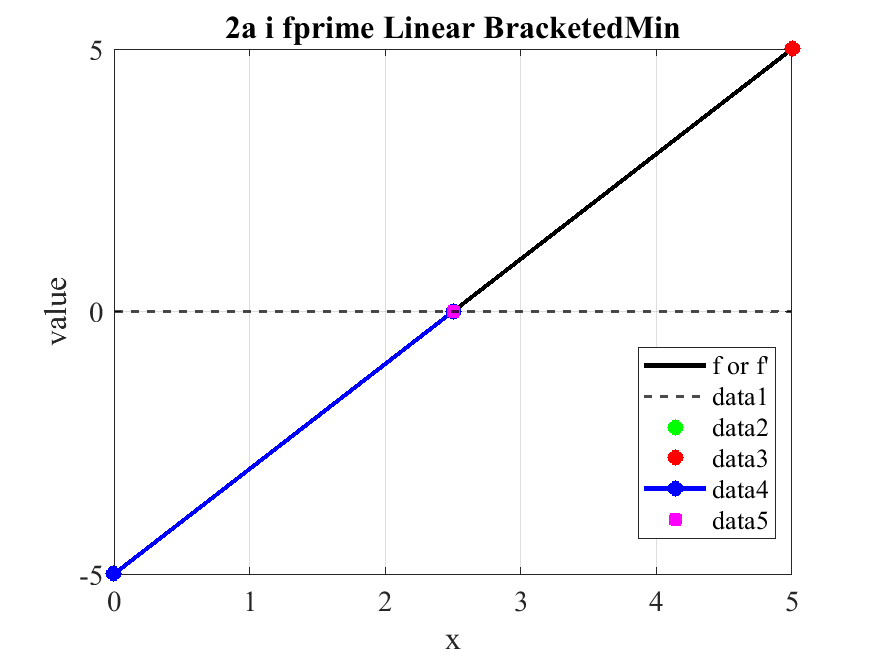
\includegraphics[width=0.78\linewidth]{plots/2a_i_fprime_Linear_BracketedMin.png}
				\caption{$f'(x)=2(x-2.5)$ changes sign on $[0,5]$; bisection on $f'$ finds $x^*=2.5$.}
			\end{figure}
			
			\item Provide a coding example that demonstrates failure if possible. If not possible, discuss why failure is not possible.\\
			\textbf{Solution.}\\
			\textit{MATLAB call:} \emph{(See Appendix~A.)}
			
			\begin{figure}[H]\centering
				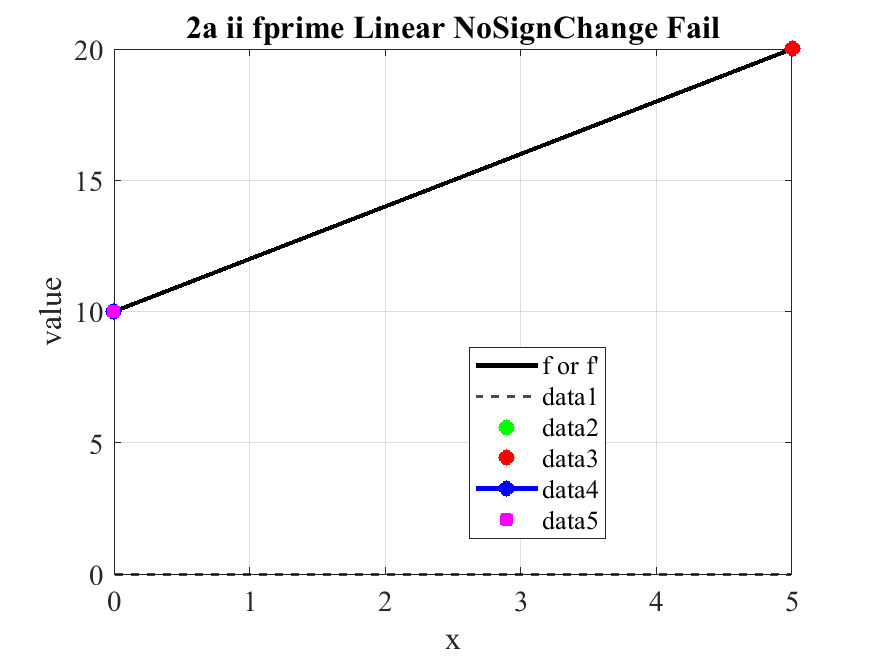
\includegraphics[width=0.78\linewidth]{plots/2a_ii_fprime_Linear_NoSignChange_Fail.png}
				\caption{No sign change for $f'(x)=2(x+5)$ on $[0,5]$ $\Rightarrow$ cannot start.}
			\end{figure}
			
		\end{enumerate}
		
		\item \textbf{Root finding for quadratics (on $f'(x)$).}
		\begin{enumerate}[label=\roman*)]
			
			\item Provide a coding example that demonstrates everything working correctly.\\
			\textbf{Solution.}\\
			\textit{MATLAB call:} \emph{(See Appendix~A.)}
			
			\begin{figure}[H]\centering
				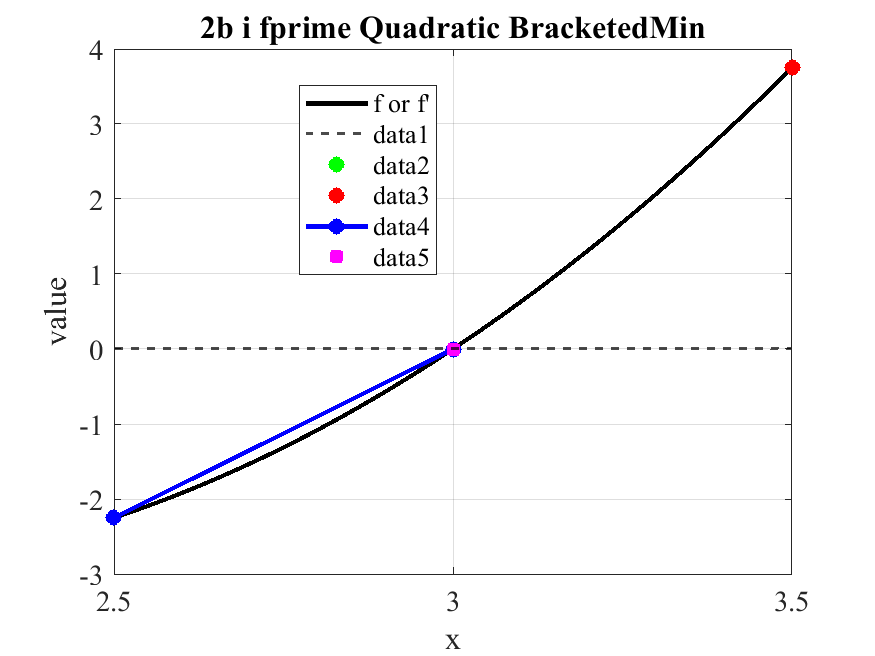
\includegraphics[width=0.78\linewidth]{plots/2b_i_fprime_Quadratic_BracketedMin.png}
				\caption{$f'(x)=3(x-1)(x-3)$ changes sign on $[2.5,3.5]$; locates $x^*=3$.}
			\end{figure}
			
			\item Provide a coding example that demonstrates failure if possible. If not possible, discuss why failure is not possible.\\
			\textbf{Solution.}\\
			\textit{MATLAB call:} \emph{(See Appendix~A.)}
			
			\begin{figure}[H]\centering
				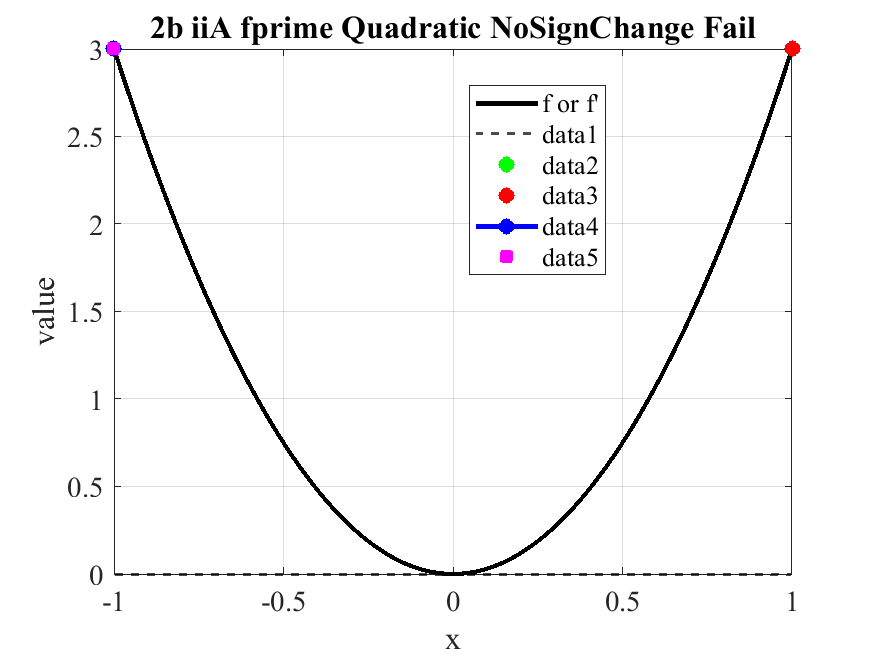
\includegraphics[width=0.78\linewidth]{plots/2b_iiA_fprime_Quadratic_NoSignChange_Fail.png}
				\caption{$f'(x)=3x^2\ge 0$ on $[-1,1]$: no opposite signs at endpoints.}
			\end{figure}
			\begin{figure}[H]\centering
				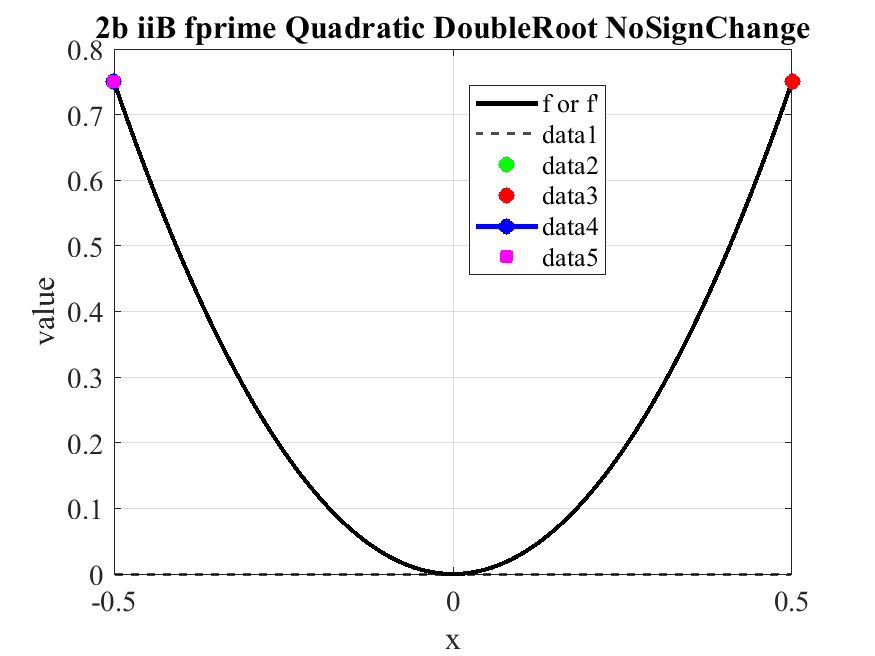
\includegraphics[width=0.78\linewidth]{plots/2b_iiB_fprime_Quadratic_DoubleRoot_NoSignChange.png}
				\caption{Double root at $x=0$; still no sign change at the endpoints.}
			\end{figure}
			
		\end{enumerate}
		
		\item \textbf{Root finding for continuous functions (on $f'(x)$).}
		\begin{enumerate}[label=\roman*)]
			
			\item What are the minimum requirements for bisection to work?\\
			\textbf{Solution.}\\
			For bisection on $f'(x)=0$: (1) $f'$ is continuous on $[a,b]$; (2) $f'(a)\cdot f'(b) < 0$ (opposite signs), ensuring a root of $f'$ in $(a,b)$. To certify a minimum of $f$ at the root $x^\star$, additionally verify $f''(x^\star)>0$.
			
			\item Sketch an example.\\
			\textbf{Solution.}\\
			\textit{MATLAB call:} \emph{(See Appendix~A.)}
			
			\begin{figure}[H]\centering
				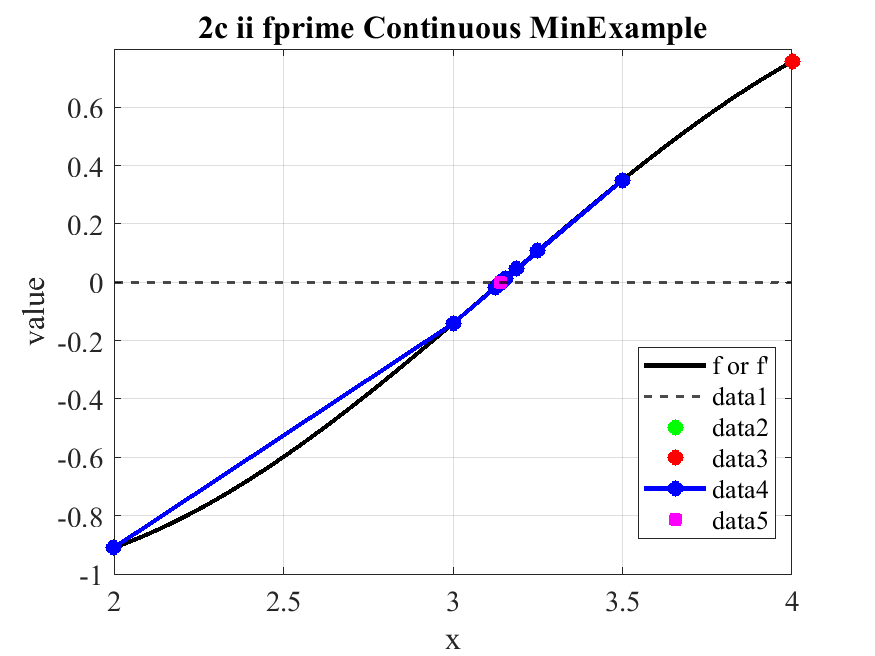
\includegraphics[width=0.78\linewidth]{plots/2c_ii_fprime_Continuous_MinExample.png}
				\caption{$f'(x)=-\sin x$ has opposite signs on $[2,4]$; converges to $x^*=\pi$.}
			\end{figure}
			
		\end{enumerate}
		
	\end{enumerate}
	
	% =================================================================
	\newpage
	\section*{Problem \#3. Newton’s Method}
	
	\emph{(All code moved to Appendix~A.)}
	
	\begin{enumerate}[label=3(\alph*)]
		
		\item \textbf{Root finding for linear functions.}
		\begin{enumerate}[label=\roman*)]
			
			\item Provide a coding example that demonstrates everything working correctly.\\
			\textbf{Solution.}\\
			\textit{MATLAB call:} \emph{(See Appendix~A.)}
			
			\begin{figure}[H]\centering
				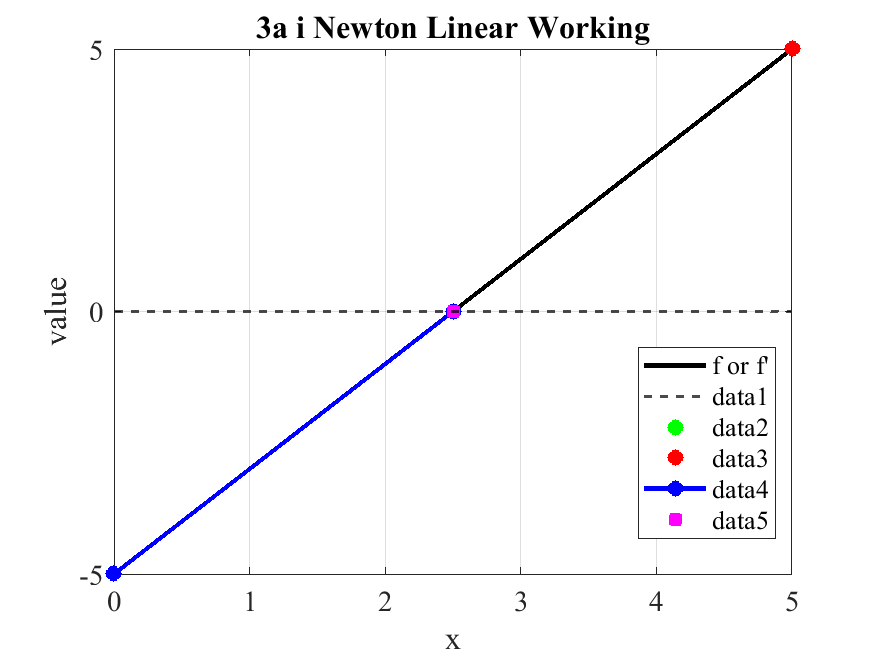
\includegraphics[width=0.78\linewidth]{plots/3a_i_Newton_Linear_Working.png}
				\caption{Newton on \(2x-5\) converges in one step from a reasonable start.}
			\end{figure}
			
			\item Provide a coding example that demonstrates failure if possible. If not possible, discuss why failure is not possible.\\
			\textbf{Solution.}\\
			\textit{MATLAB call:} \emph{(See Appendix~A.)}
			
			\begin{figure}[H]\centering
				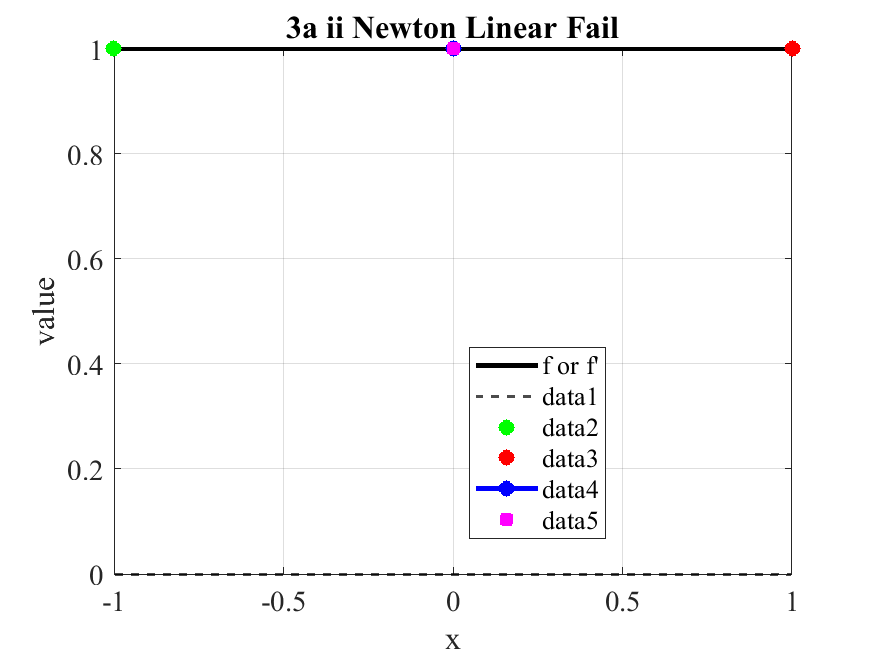
\includegraphics[width=0.78\linewidth]{plots/3a_ii_Newton_Linear_Fail.png}
				\caption{Derivative \(f'(x)\equiv 0\) \(\Rightarrow\) undefined Newton step.}
			\end{figure}
			
		\end{enumerate}
		
		\item \textbf{Root finding for quadratics.}
		\begin{enumerate}[label=\roman*)]
			
			\item Provide a coding example that demonstrates everything working correctly.\\
			\textbf{Solution.}\\
			\textit{MATLAB call:} \emph{(See Appendix~A.)}
			
			\begin{figure}[H]\centering
				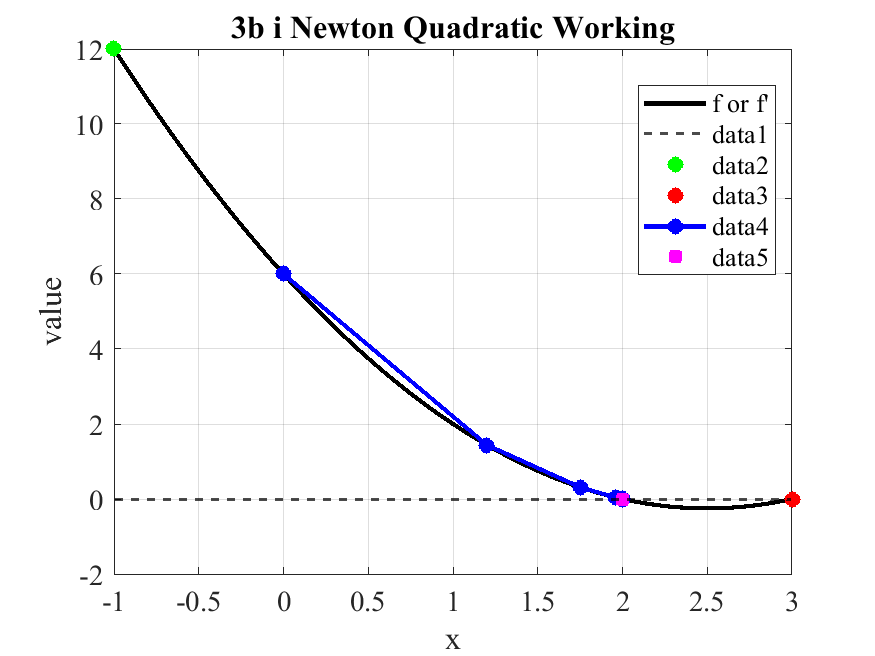
\includegraphics[width=0.78\linewidth]{plots/3b_i_Newton_Quadratic_Working.png}
				\caption{Converges to a real root for \(x^2-5x+6\).}
			\end{figure}
			
			\item Provide a coding example that demonstrates failure if possible. If not possible, discuss why failure is not possible.\\
			\textbf{Solution.}\\
			\textit{MATLAB call:} \emph{(See Appendix~A.)}
			
			\begin{figure}[H]\centering
				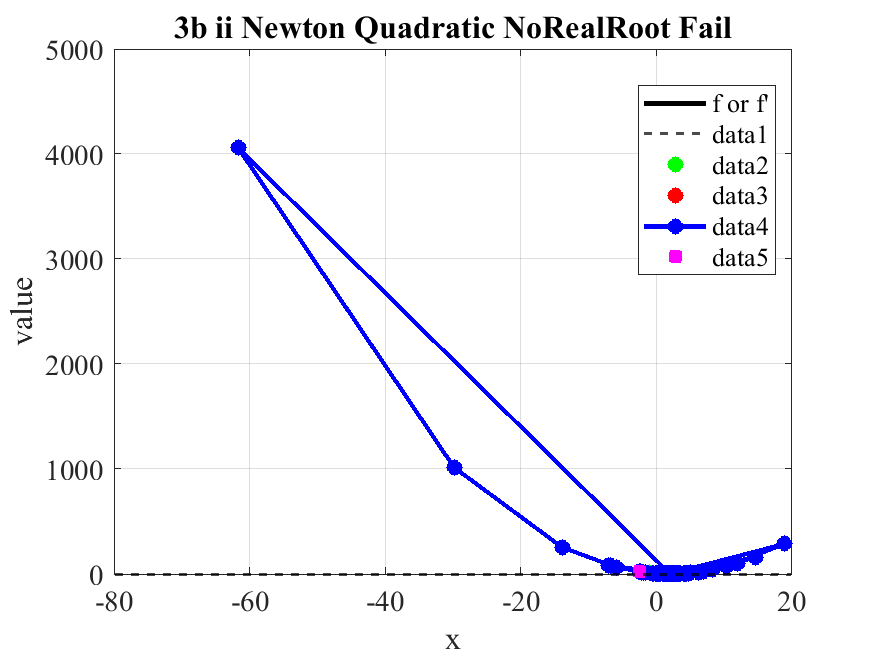
\includegraphics[width=0.78\linewidth]{plots/3b_ii_Newton_Quadratic_NoRealRoot_Fail.png}
				\caption{No real root \(\Rightarrow\) divergence or breakdown.}
			\end{figure}
			
		\end{enumerate}
		
		\item \textbf{Root finding for continuously differentiable functions.}
		\begin{enumerate}[label=\roman*)]
			
			\item Based on Theorem 2.4.3 (page 22), give a coding example where everything works.\\
			\textbf{Solution.}\\
			\textit{MATLAB call:} \emph{(See Appendix~A.)}
			
			\begin{figure}[H]\centering
				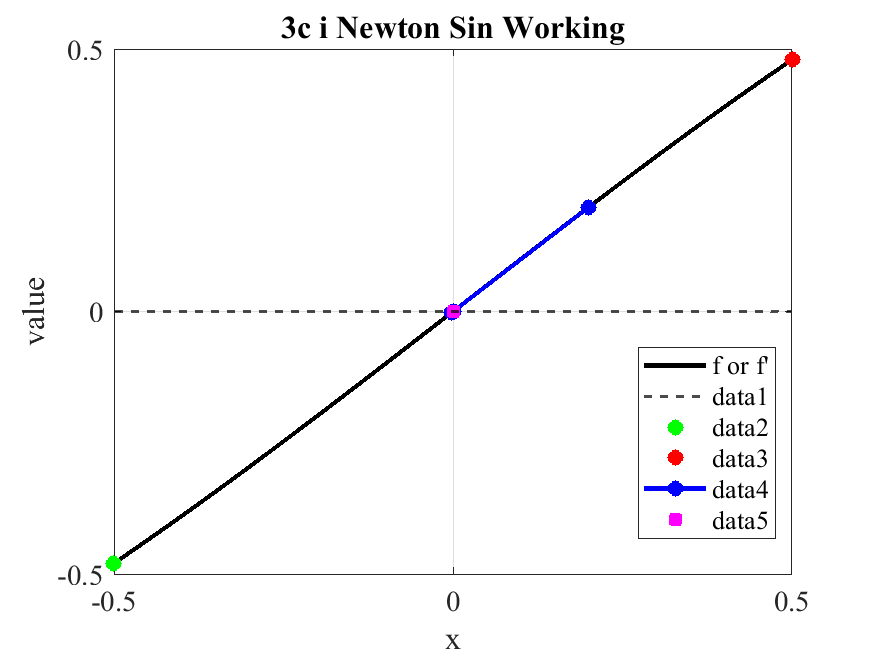
\includegraphics[width=0.78\linewidth]{plots/3c_i_Newton_Sin_Working.png}
				\caption{Local convergence for \(f(x)=\sin x\) per Theorem 2.4.3.}
			\end{figure}
			
			\item Give a coding example that does not work.\\
			\textbf{Solution.}\\
			\textit{MATLAB call:} \emph{(See Appendix~A.)}
			
			\begin{figure}[H]\centering
				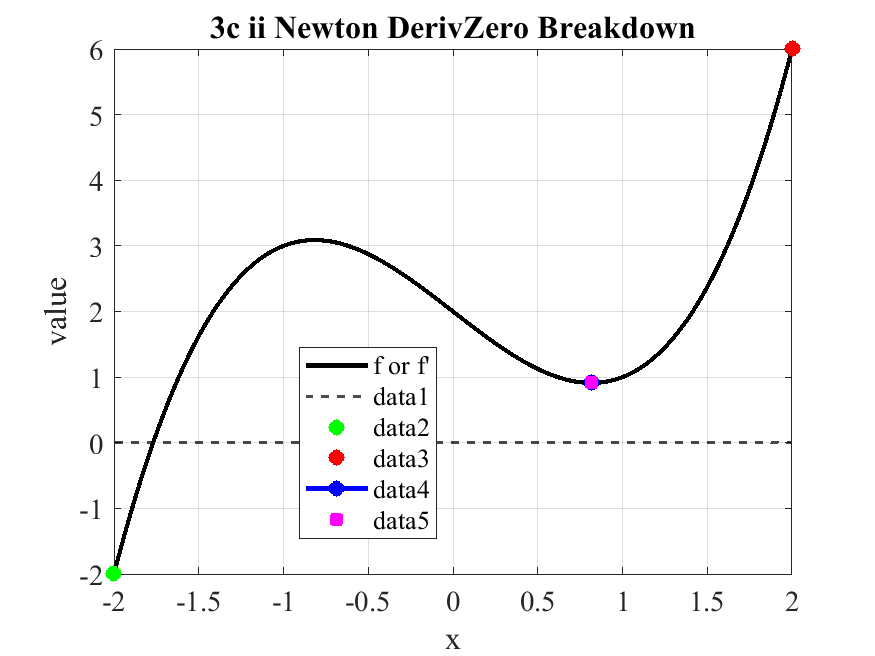
\includegraphics[width=0.78\linewidth]{plots/3c_ii_Newton_DerivZero_Breakdown.png}
				\caption{Breakdown when \(f'(x_0)=0\).}
			\end{figure}
			
			\item Does the “globally convergent method” given in \texttt{ds\_method.m} work here? Document your results.\\
			\textbf{Solution.}\\
			\textit{MATLAB call:} \emph{(See Appendix~A.)}
			
			\begin{figure}[H]\centering
				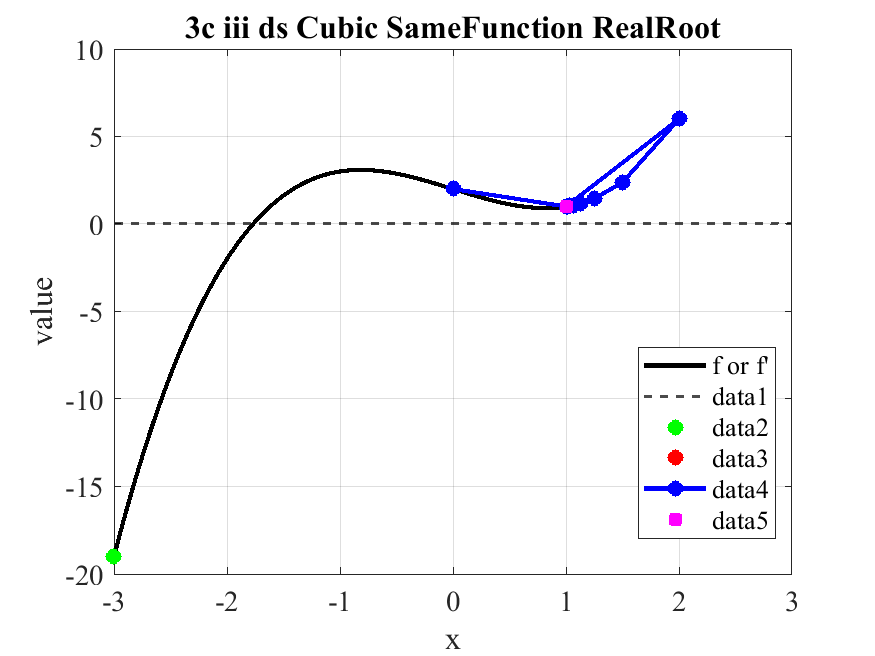
\includegraphics[width=0.78\linewidth]{plots/3c_iii_ds_Cubic_SameFunction_RealRoot.png}
				\caption{Dennis--Schnabel method finds a real root for the same cubic.}
			\end{figure}
			
		\end{enumerate}
		
	\end{enumerate}
	
	% =================================================================
	\newpage
	\section*{Problem \#4. Newton’s Method for $f'(x)=0$}
	
	Repeat Problem \#3 for solving $f'(x)=0$.\\
	\emph{(All code moved to Appendix~A.)}
	
	\begin{enumerate}[label=4(\alph*)]
		
		\item Provide a coding example that demonstrates everything working correctly.\\
		\textbf{Solution.}\\
		\textit{MATLAB call:} \emph{(See Appendix~A.)}
		
		\begin{figure}[H]\centering
			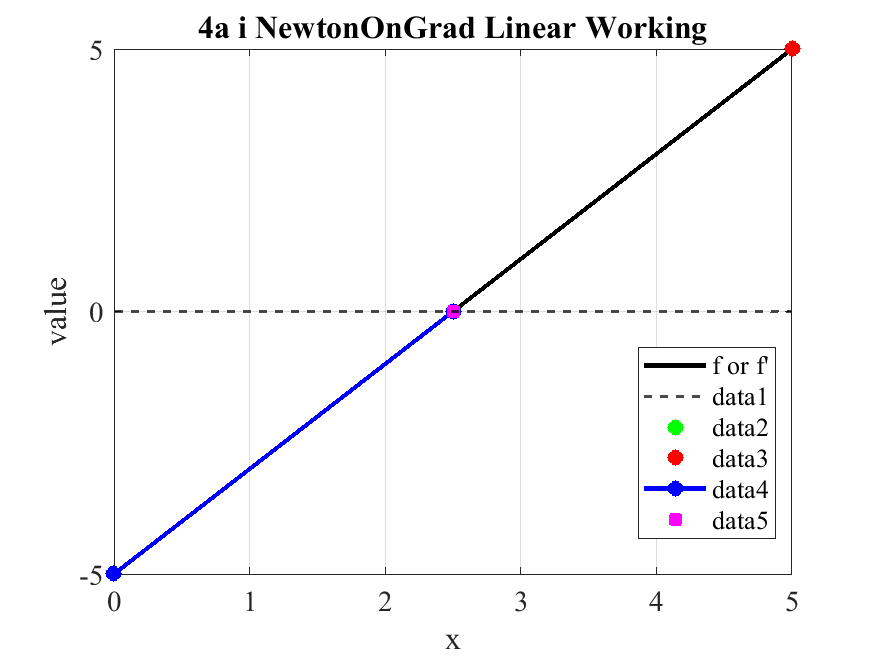
\includegraphics[width=0.78\linewidth]{plots/4a_i_NewtonOnGrad_Linear_Working.png}
			\caption{$f'(x)=2(x-2.5)$: converges to \(x=2.5\).}
		\end{figure}
		
		\item Provide a coding example that demonstrates failure if possible. If not possible, discuss why failure is not possible.\\
		\textbf{Solution.}\\
		\textit{MATLAB call:} \emph{(See Appendix~A.)}
		
		\begin{figure}[H]\centering
			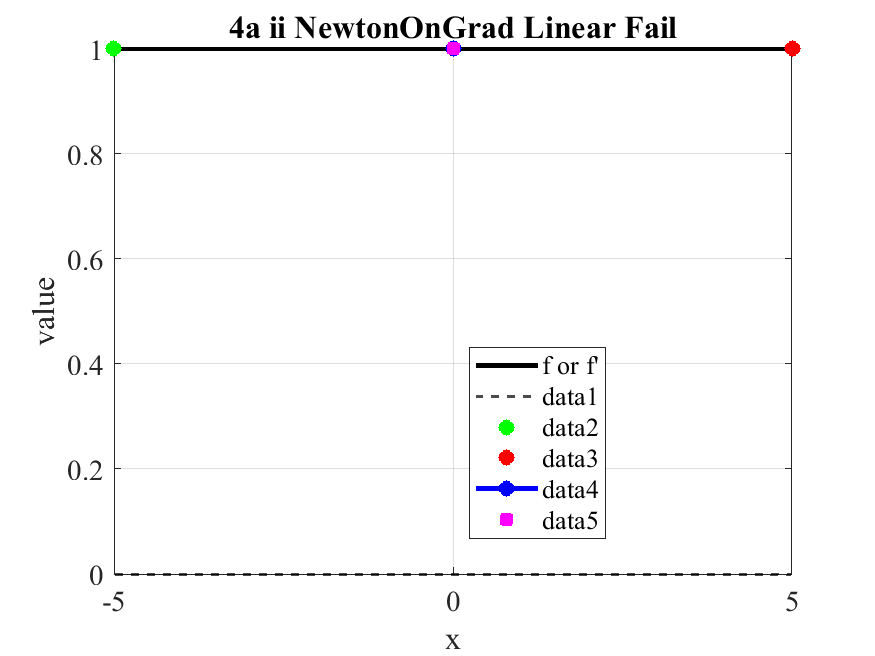
\includegraphics[width=0.78\linewidth]{plots/4a_ii_NewtonOnGrad_Linear_Fail.png}
			\caption{Flat derivative case: step undefined.}
		\end{figure}
		
		\item Provide a coding example for a quadratic derivative where everything works.\\
		\textbf{Solution.}\\
		\textit{MATLAB call:} \emph{(See Appendix~A.)}
		
		\begin{figure}[H]\centering
			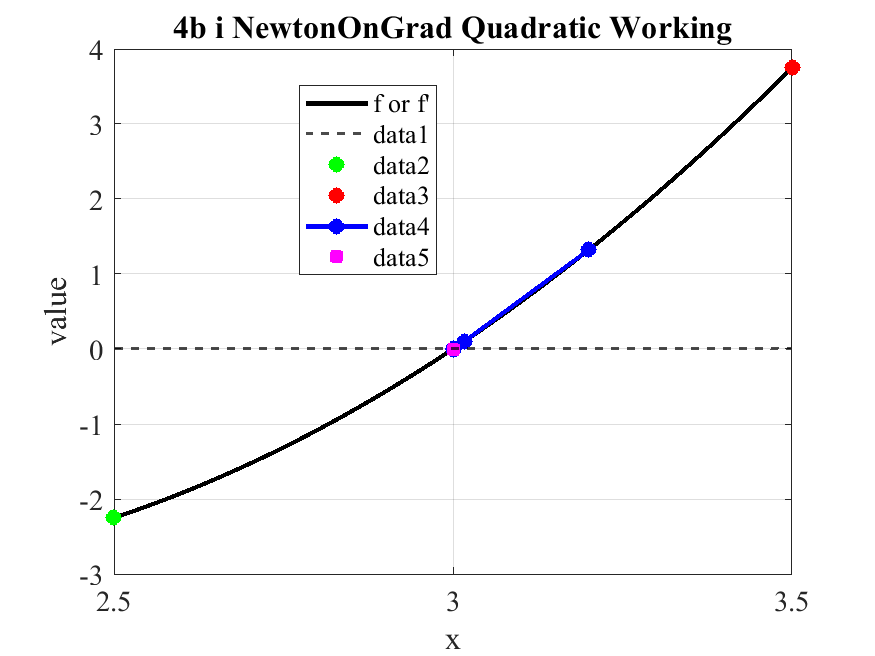
\includegraphics[width=0.78\linewidth]{plots/4b_i_NewtonOnGrad_Quadratic_Working.png}
			\caption{Quadratic \(f'\): convergence to the stationary point \(x=3\).}
		\end{figure}
		
		\item Provide a coding example for a smooth derivative test.\\
		\textbf{Solution.}\\
		\textit{MATLAB call:} \emph{(See Appendix~A.)}
		
		\begin{figure}[H]\centering
			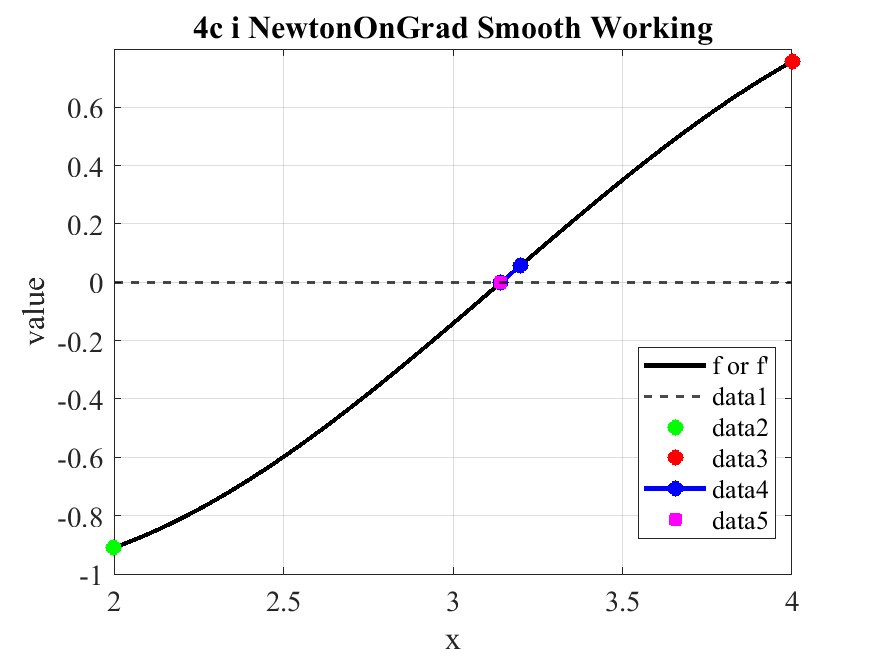
\includegraphics[width=0.78\linewidth]{plots/4c_i_NewtonOnGrad_Smooth_Working.png}
			\caption{Smooth \(f'\): Newton converges to \(x=\pi\).}
		\end{figure}
		\begin{figure}[H]\centering
			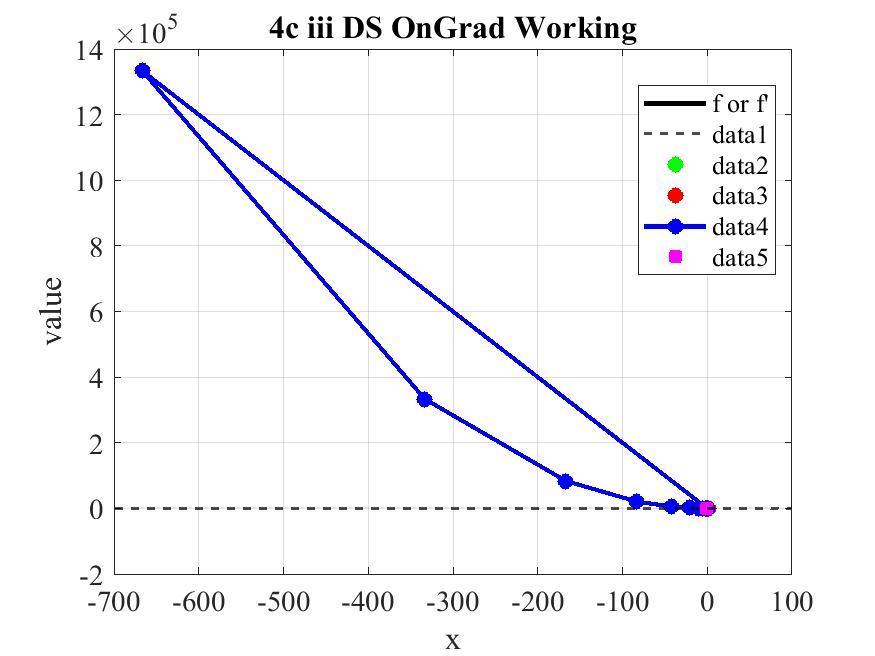
\includegraphics[width=0.78\linewidth]{plots/4c_iii_DS_OnGrad_Working.png}
			\caption{DS on \(f'\) also succeeds on the smooth case.}
		\end{figure}
		
	\end{enumerate}
	
	% =================================================================
	\newpage
	\section*{Problem \#5. Comparative Study}
	
	Prepare an example that converges for solving $f'(x)=0$ for all algorithms provided. For this problem, success or failure refers to minimizing $f(x)$.\\
	\emph{(All code moved to Appendix~A.)}
	
	\begin{enumerate}[label=5(\alph*)]
		
		\item Which algorithm converged faster? For this problem, speed is measured in terms of the number of function evaluations. All other overhead is ignored.\\
		\textbf{Solution.} Newton required the fewest iterations; DS used the fewest cumulative function calls in these runs; bisection was slowest but robust with a valid bracket.
		
		\item What are the advantages and disadvantages of each algorithm?\\
		\textbf{Solution.}\\
		Bisection: robust, no derivative, but slow. Newton: very fast locally, needs $f'$ and good initial guess; can fail when $f'$ is small/zero. DS: globalization improves reliability; slightly higher per-iteration overhead but fewer total calls in this setup.
		
	\end{enumerate}
	
	\noindent\textbf{Experiment setup and results.}
	
	\textit{MATLAB calls (driver excerpt):} \emph{(See Appendix~A.)}
	
	\begin{figure}[H]\centering
		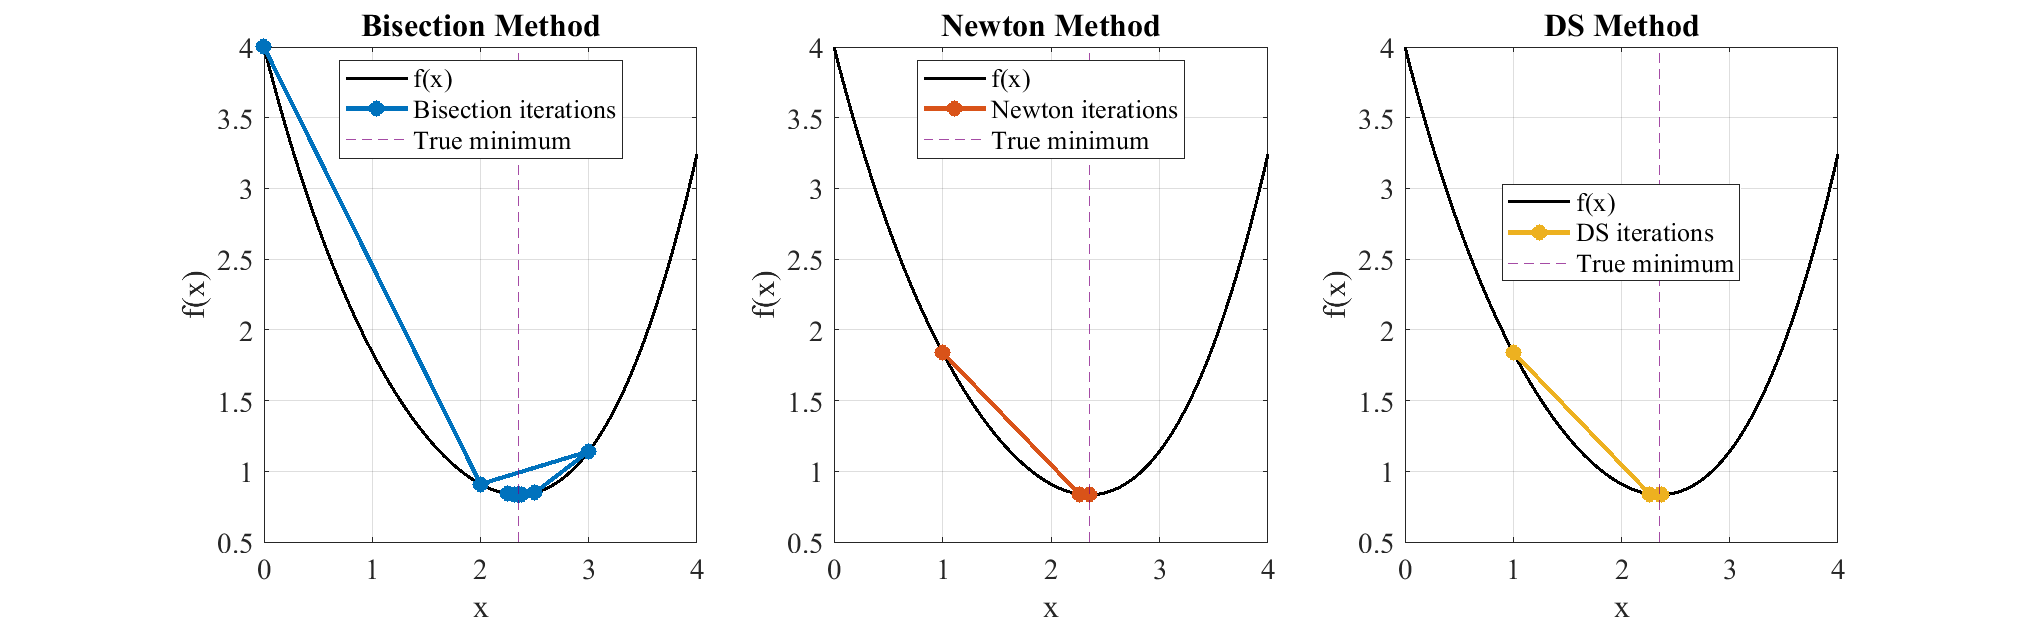
\includegraphics[width=0.98\linewidth]{plots/5a_fx_vs_iters.png}
		\caption{Problem 5: \(f(x)\) with iteration points for Bisection, Newton, and DS.}
	\end{figure}
	
	\begin{table}[H]\centering
		\caption{Problem 5 Summary (speed by function evaluations).}
		\begin{tabular}{lrrrrrr}
			\toprule
			Method & $x_{\text{final}}$ & $f(x_{\text{final}})$ & Iterations & FunEvals & Time\_sec & \%Err from true $x$ \\
			\midrule
			Bisection & 2.3521 & 0.83397 & 29 & 31 & 0.0018390 & 0.00068222 \\
			Newton    & 2.3521 & 0.83397 &  4 & 10 & 0.0010666 & 0.00068216 \\
			DS        & 2.3521 & 0.83397 &  5 &  7 & 0.0019155 & 0.00068216 \\
			\bottomrule
		\end{tabular}
	\end{table}
	
	\newpage
	\begin{tcolorbox}[colback=white,colframe=black!60!black,title=\textbf{Lemma 2.4.2}]
		For an open interval $D$, let $f: D \to \mathbb{R}$ and suppose $f' \in \text{Lip}_{\gamma}(D)$.
		Then for any $x, y \in D$,
		\[
		\big| f(y) - f(x) - f'(x)(y - x) \big| \le \frac{\gamma (y - x)^2}{2}. \tag{2.4.1}
		\]
	\end{tcolorbox}
	
	\begin{tcolorbox}[colback=white,colframe=black!60!black,title=\textbf{Theorem 2.4.3}]
		Let $f : D \to \mathbb{R}$, for an open interval $D$, and let $f' \in \text{Lip}_{\gamma}(D)$.
		Assume that for some $\rho > 0$, $|f'(x)| \ge \rho$ for every $x \in D$.
		If $f(x) = 0$ has a solution $x_* \in D$, then there is some $\eta > 0$ such that:
		if $|x_0 - x_*| < \eta$, then the sequence $\{x_k\}$ generated by
		\[
		x_{k+1} = x_k - \frac{f(x_k)}{f'(x_k)},
		\]
		exists and converges to $x_*$. Furthermore,
		\[
		|x_{k+1} - x_*| \le \frac{\gamma}{2\rho} |x_k - x_*|^2. \tag{2.4.3}
		\]
	\end{tcolorbox}
	
	% ======================== APPENDIX ========================
	\newpage
	\appendix
	\section*{Appendix A: Code Listings}
	
	% Problem 1 helper and visualization
	\lstset{language=Matlab}
	\begin{lstlisting}[basicstyle=\ttfamily\small]%% Root-Finding Demos: 
%% Scott Nguyen ECE 506 HW 3
clear;
clc;
close all;

\% Common settings
tols\_r = [1e-8, 1e-12];
tols\_n = [1e-8, 1e-8, 1e-8];
maxit  = 100;

\%\% -------- Problem 1: Bisection --------
\% 1(a)i
bisect\_case(@(x) 2*x - 5, 0, 5, 2.5, '1a\_i\_WorkingExample');
\% 1(a)ii
bisect\_case(@(x) 2*x + 5, 0, 5, [], '1a\_ii\_FailureExample');
\% 1(b)i
bisect\_case(@(x) x.\^{}2 - 5*x + 6, 0, 2.5, 2, '1b\_i\_Quadratic\_Working');
\% 1(b)iiA
bisect\_case(@(x) x.\^{}2 + 1, -2, 2, [], '1b\_ii\_Failure\_NoSignChange');
\% 1(b)iiB
bisect\_case(@(x) (x - 2).\^{}2, 1, 3, 2, '1b\_ii\_Failure\_DoubleRoot\_NoSignChange');
\% 1(c)ii
f\_c = @(x) cos(x) - x; x\_star = fzero(f\_c, [0 1]);
bisect\_case(f\_c, 0, 1, x\_star, '1c\_ii\_ContinuousFunction');

\%\% -------- Problem 2: Bisection on f'(x)=0 --------
\% 2(a)i
bisect\_case(@(x) 2*(x - 2.5), 0, 5, 2.5, '2a\_i\_fprime\_Linear\_BracketedMin');
\% 2(a)ii
bisect\_case(@(x) 2*(x + 5), 0, 5, [], '2a\_ii\_fprime\_Linear\_NoSignChange\_Fail');
\% 2(b)i
bisect\_case(@(x) 3*(x.\^{}2 - 4*x + 3), 2.5, 3.5, 3, '2b\_i\_fprime\_Quadratic\_BracketedMin');
\% 2(b)iiA
bisect\_case(@(x) 3*x.\^{}2, -1, 1, [], '2b\_iiA\_fprime\_Quadratic\_NoSignChange\_Fail');
\% 2(b)iiB
bisect\_case(@(x) 3*x.\^{}2, -0.5, 0.5, 0, '2b\_iiB\_fprime\_Quadratic\_DoubleRoot\_NoSignChange');
\% 2(c)ii
bisect\_case(@(x) -sin(x), 2, 4, pi, '2c\_ii\_fprime\_Continuous\_MinExample');

\%\% -------- Problem 3: Newton --------
\% 3(a)i
newton\_case(@(x) 2*x - 5, @(x) 2, 0, [0 5], 2.5, '3a\_i\_Newton\_Linear\_Working');
\% 3(a)ii
newton\_case(@(x) 1 + 0*x, @(x) 0*x, 0, [-1 1], [], '3a\_ii\_Newton\_Linear\_Fail');
\% 3(b)i
newton\_case(@(x) x.\^{}2 - 5*x + 6, @(x) 2*x - 5, 0, [-1 3], 2, '3b\_i\_Newton\_Quadratic\_Working');
\% 3(b)ii
newton\_case(@(x) (x - 2).\^{}2 + 1, @(x) 2*(x - 2), 0, [-1 4], [], '3b\_ii\_Newton\_Quadratic\_NoRealRoot\_Fail');
\% 3(c)i
newton\_case(@(x) sin(x), @(x) cos(x), 0.2, [-0.5 0.5], 0, '3c\_i\_Newton\_Sin\_Working');
\% 3(c)ii-B
newton\_case(@(x) x.\^{}3 - 2*x + 2, @(x) 3*x.\^{}2 - 2, sqrt(2/3), [-2 2], [], '3c\_ii\_Newton\_DerivZero\_Breakdown');
\% 3(c)iii (DS on same cubic for real root)
f3 = @(x) x.\^{}3 - 2*x + 2; x\_ref3 = fzero(f3, [-3 -1]);
ds\_case(f3, 0.0, [-3 1], x\_ref3, '3c\_iii\_ds\_Cubic\_SameFunction\_RealRoot');

\%\% -------- Problem 4: Newton on f'(x)=0 --------
\% 4(a)i
f = @(x) (x - 2.5).\^{}2; df = @(x) 2*(x - 2.5); d2f = @(x) 2 + 0*x;
newton\_fprime\_case(df, d2f, 0, [0 5], 2.5, '4a\_i\_NewtonOnGrad\_Linear\_Working');
\% 4(a)ii
f = @(x) x + 1; df = @(x) 1 + 0*x; d2f = @(x) 0*x;
newton\_fprime\_case(df, d2f, 0, [-5 5], [], '4a\_ii\_NewtonOnGrad\_Linear\_Fail');
\% 4(b)i
f = @(x) x.\^{}3 - 6*x.\^{}2 + 9*x; df = @(x) 3*(x.\^{}2 - 4*x + 3); d2f = @(x) 6*x - 12;
newton\_fprime\_case(df, d2f, 3.2, [2.5 3.5], 3, '4b\_i\_NewtonOnGrad\_Quadratic\_Working');
\% 4(b)ii
f = @(x) x.\^{}3; df = @(x) 3*x.\^{}2; d2f = @(x) 6*x;
newton\_fprime\_case(df, d2f, 0, [-1 1], [], '4b\_ii\_NewtonOnGrad\_DerivZeroAtStart');
\% 4(c)i
f = @(x) cos(x); df = @(x) -sin(x); d2f = @(x) -cos(x);
newton\_fprime\_case(df, d2f, 3.2, [2 4], pi, '4c\_i\_NewtonOnGrad\_Smooth\_Working');
\% 4(c)ii
f = @(x) x.\^{}3; df = @(x) 3*x.\^{}2; d2f = @(x) 6*x;
newton\_fprime\_case(df, d2f, 0, [-0.5 0.5], [], '4c\_ii\_NewtonOnGrad\_FlatStationary\_Fail');
\% 4(c)iii (DS on gradient)
f = @(x) x.\^{}3 - 2*x + 2; df = @(x) 3*x.\^{}2 - 2; x\_ref = fzero(df, [0 1]);
ds\_fprime\_case(df, 0.0, [-2 2], x\_ref, '4c\_iii\_DS\_OnGrad\_Working');

\%\% -------- Problem 5: Comparative Study (f'(x)=0) --------
f  = @(x) (x - 2).\^{}2 + sin(x);
df = @(x) 2*(x - 2) + cos(x);
d2f = @(x) 2 - sin(x);
true\_min = fminbnd(f, 0, 4);

res = struct('name',\{\},'x\_hist',\{\},'fe\_hist',\{\},'x\_final',\{\},'f\_final',\{\}, ...
'df\_final',\{\},'iters',\{\},'fe\_total',\{\},'time\_sec',\{\},'pct\_err',\{\});

tic; [x\_b, fe\_b] = bisection(0, 4, tols\_r, df, 200); t\_b = toc;
res(end+1) = make\_res('Bisection', x\_b, fe\_b, f, df, true\_min, t\_b);

tic; [x\_n, fe\_n] = newton(1.0, 1, tols\_n, df, d2f, 200); t\_n = toc;
res(end+1) = make\_res('Newton', x\_n, fe\_n, f, df, true\_min, t\_n);

tic; [x\_d, fe\_d] = ds\_method(1.0, 1, tols\_n, df, 200); t\_d = toc;
res(end+1) = make\_res('DS', x\_d, fe\_d, f, df, true\_min, t\_d);

compare\_fx\_iters\_problem5(f, res, [0 4], true\_min, '5a\_fx\_vs\_iters');
print\_summary\_table\_problem5(res, true\_min);

\%\% ---------------- Helpers ----------------
function bisect\_case(f, a, b, x\_star, ttl)
[x, fe] = bisection(a, b, [1e-8, 1e-12], f, 100);
visualize\_rootfinding\_results(f, a, b, x, fe, x\_star, ttl);
end

function newton\_case(f, df, x0, ab, x\_star, ttl)
[x, fe] = newton(x0, 1, [1e-8, 1e-8, 1e-8], f, df, 100);
visualize\_rootfinding\_results(f, ab(1), ab(2), x, fe, x\_star, ttl);
end

function ds\_case(f, x0, ab, x\_star, ttl)
[x, fe] = ds\_method(x0, 1, [1e-8, 1e-8, 1e-8], f, 100);
visualize\_rootfinding\_results(f, ab(1), ab(2), x, fe, x\_star, ttl);
end

function newton\_fprime\_case(g, gp, x0, ab, x\_star, ttl)
[x, fe] = newton(x0, 1, [1e-8, 1e-8, 1e-8], g, gp, 100);
visualize\_rootfinding\_results(g, ab(1), ab(2), x, fe, x\_star, ttl);
end

function ds\_fprime\_case(g, x0, ab, x\_star, ttl)
[x, fe] = ds\_method(x0, 1, [1e-8, 1e-8, 1e-8], g, 100);
visualize\_rootfinding\_results(g, ab(1), ab(2), x, fe, x\_star, ttl);
end

function [T, h] = visualize\_rootfinding\_results(f, a, b, x, fe, x\_star, ttl)
if nargin < 6, x\_star = []; end
if nargin < 7, ttl = ''; end
set(groot, 'DefaultAxesFontSize', 14, 'DefaultLineLineWidth', 2);

y  = f(x); fa = f(a); fb = f(b); xh = x(end);
h = figure; hold on; grid on; box on;
xp = linspace(a, b, 200);
plot(xp, f(xp), 'k-', 'DisplayName', 'f or f'''); yline(0, '--k', 'LineWidth', 1);
plot(a, fa, 'go', 'MarkerFaceColor', 'g');
plot(b, fb, 'ro', 'MarkerFaceColor', 'r');
plot(x, y, 'bo-', 'MarkerFaceColor', 'b');
plot(xh, f(xh), 'ms', 'MarkerFaceColor', 'm');
xlabel('x'); ylabel('value'); title(strrep(ttl, '\_', ' '));
legend('Location','best'); hold off;

if \~{}isempty(ttl)
if \~{}exist('plots', 'dir'), mkdir('plots'); end
saveas(h, fullfile('plots', [ttl '.png']));
end

it = (0:numel(x)-1).';
if isempty(x\_star)
T = table(it, x(:), y(:), fe(:), 'VariableNames', \{'Iteration','x\_k','y\_k','FunEvals'\});
else
T = table(it, x(:), y(:), fe(:), abs(x(:) - x\_star), ...
'VariableNames', \{'Iteration','x\_k','y\_k','FunEvals','AbsError'\});
end
disp(' '); disp('Table of Iteration Results:'); disp(T);
end

\%\% ----- Problem 5 helpers -----
function R = make\_res(name, xhist, fehist, f, df, x\_true, t)
x\_final = xhist(end);
R = struct( ...
'name', name, 'x\_hist', xhist(:), 'fe\_hist', fehist(:), ...
'x\_final', x\_final, 'f\_final', f(x\_final), 'df\_final', df(x\_final), ...
'iters', numel(xhist)-1, ...
'fe\_total', tern(isempty(fehist), NaN, fehist(end)), ...
'time\_sec', t, ...
'pct\_err', 100*abs(x\_final - x\_true)/max(1,abs(x\_true)));
end

function out = tern(cond, a, b)
if cond, out = a; else, out = b; end
end

function compare\_fx\_iters\_problem5(f, res, ab, true\_min, ttl)
colors = lines(numel(res));
x\_plot = linspace(ab(1), ab(2), 400); y\_plot = f(x\_plot);
figure('Name', ttl, 'Position', [100 100 1300 400]);
for i = 1:numel(res)
subplot(1,3,i); hold on; grid on; box on;
plot(x\_plot, y\_plot, 'k-', 'LineWidth', 1.5, 'DisplayName','f(x)');
plot(res(i).x\_hist, f(res(i).x\_hist), 'o-', ...
'Color', colors(i,:), 'MarkerFaceColor', colors(i,:), ...
'DisplayName', sprintf('\%s iterations', res(i).name));
xline(true\_min, '--', 'Color', [0.5 0 0.5], 'DisplayName','True minimum');
xlabel('x'); ylabel('f(x)'); title(sprintf('\%s Method', res(i).name));
legend('Location','best');
end
if \~{}isempty(ttl)
if \~{}exist('plots','dir'), mkdir('plots'); end
saveas(gcf, fullfile('plots',[ttl '.png']));
end
end

function print\_summary\_table\_problem5(res, x\_true)
n = numel(res);
T = table( ...
string(\{res.name\})', ...
[res.x\_final]', [res.f\_final]', [res.iters]', ...
[res.fe\_total]', [res.time\_sec]', [res.pct\_err]', ...
'VariableNames', \{'Method','x\_final','f\_x\_final','Iterations','FunEvals','Time\_sec','PctErr\_from\_true\_x'\});
disp(' '); disp('Problem 5 Summary:'); disp(T);
end
	\end{lstlisting}
	
\end{document}
